\subsection{تابع الانتباه\label{att}}
كما ذكرنا في الفقرات السابقة فإن تابع الانتباه هو الجزء الأساسي في نموذج المحول، لذلك وجب شرحه بشيء من التفصيل في الفقرة الحالية، إذ سنشرح عن التابع بشكل عام وعن مفهوم الانتباه، ثم سنشرح عن طريقة استخدامه في نموذج المحول.
\subsubsection{الفكرة العامة لتابع الانتباه الذاتي 
\textLR{self-attention}
\label{section:att_example}
}
لتبسيط شرح مفهوم تابع الانتباه الذاتي سنقوم بالاستعانة بمثال بسيط عن الترجمة، إذ يمكن إسقاط هذا المثال على مجالات أخرى كالرؤية الحاسوبية، وذلك باعتبار $"$الكلمة$"$ مقابلة لـ $"$البكسل$"$ أو $"$مجموعة من البكسلات$"$.
\newline
لنأخذ كمثال جملة 
\textLR{Bank of a river}.
\newline
بداية نحول كل كلمة إلى تمثيل رقمي ندعوه بالـ
\textLR{token}
عبر
\textLR{word embedding}.
هناك العديد من الخوارزميات المدربة مسبقاً لهذا الغرض، بحيث تكون الكلمات المتشابهة بالمعنى $"$متشابهة$"$ أيضاً بالتمثيل الرقمي (أي أن الجداء السلمي لها قيمة قريبة من الواحد). عندها يمكن تمثيل الجملة السابقة كما يلي:
\newline
\textLR{Bank of a river}
\newline
$[word_1, word_2, word_3, word_4]$
\newline
بعد تحويل الـ
\textLR{embedding}
\newline
$X = [x_1,x_2,x_3,x_4]$
\newline
كما ذكرنا سابقاً هدف الانتباه هو تعديل شعاع الـ
\textLR{embedding}
ليناسب السياق. سنشرح فيما يلي كيف يتم ذلك.
\newline
أولاً نحسب التشابه بين كل كلمة في الجملة مع كل كلمات الجملة وذلك عن طريق الجداء السلمي 
\textLR{dot-product}
كما في المعادلات
\ref{eq:att_dot_product}.
\begin{equation}
\begin{split}
&s_{11} = x_1.x_1\\
&s_{12} = x_1.x_2\\
&\text{...}\\
&s_{ij} = x_i.x_j\\
\end{split}
\label{eq:att_dot_product}
\end{equation}
نطبق
\textLR{softmax}
لجعل قيم التشابه ضمن المجال
$[0,1]$
بحيث يكون التشابه بين الكلمة $i$ وكامل الجملة كما في المعادلة 
\ref{eq:att_softmax}.
\begin{equation}
score_{i1},score_{i2},... = softmax(s_{i1},s_{i2},..)
\label{eq:att_softmax}
\end{equation}
من خلال استخدام تابع الانتباه يتم تعديل تمثيل الكلمة $x_i$  بحسب التشابه بينها وبين كلمات الجملة أي بحسب قيم الـ $score_{ij}$، فيكون التمثيل المعدل كما في المعادلة 
\ref{eq:att_fin}>
\begin{equation}
x_{i_{new}} = score_{i1}*x_1+score_{i2}*x_2+...
\label{eq:att_fin}
\end{equation}
وبهذه الطريقة يتغير تمثيل كل كلمة بحسب السياق الكامل للجملة. 
\newline
يستخدم نموذج المحول تابع انتباه مع أشعة تسمى بـ
\textLR{Query ,Keys,Values}،
هذه التسمية مستوحاة من أنظمة الاسترجاع
\textLR{retrieval systems}.
بشكل عام يكون لتابع الانتباه  شعاعا دخل
$X_1,X_2$،
يولد
$X_2$
الـ
\textLR{Query}،
ويولد
$X_1$
كل من الـ
\textLR{Key,Value}،
وذلك باستخدام مصفوفات
$W_q,W_v,W_k$
عناصرها أوزان قابلة للتدريب كما في المعادلات 
\ref{eq:att_mat}.
\begin{equation}
\begin{split}
&Q = X_2 W_q\\
&K = X_1 W_k\\
&V = X_1 W_v\\
\end{split}
\label{eq:att_mat}
\end{equation}
بالنسبة لتابع الانتباه الذاتي يكون
$X_1 = X_2$.
أما في الانتباه التقاطعي الذي سنذكره لاحقاً في الفقرة
\ref{section:attention}
فإن
$X_1$
مصدرها خرج المرمز، أما
$X_2$
فمصدرها مفكك الترميز.
\subsubsection{الانتباه\label{section:attention}}
 هناك نوعان من الانتباه في نموذج المحول، الانتباه الذاتي
\textLR{self-attention}،
والانتباه التقاطعي
\textLR{cross-attention}.
بالنسبة لتابع الانتباه الذاتي له ثلاث مداخل وهي
\textLR{Q query,K key,V value}،
هذه المصفوفات ناتجة عن ضرب مصفوفة الدخل
$X$
في كل طبقة مرمز بمصفوفات
$W_q,W_v,W_k$
 بالتسلسل كما في المعادلات
\ref{eq:att_mat}،
وعناصر هذه المصفوفات هي أوزان تحدد قيمها أثناء التدريب.
\newline
يمكن أيضاً أن نعبر عن تابع الانتباه باستخدام مصفوفات
$Q,K,V$
بالمعادلة
\ref{eq:att}
\textLR{\cite{Vaswani17}}
وكما يوضحه الشكل 
\ref{fig:att_dot_prod}.
\begin{equation}
\begin{split}
Attention(Q,K,V) = softmax(\frac{QK^T}{\sqrt{d_k}})V
\label{eq:att}
\end{split}
\end{equation}
\begin{figure}[h!]
\centerline{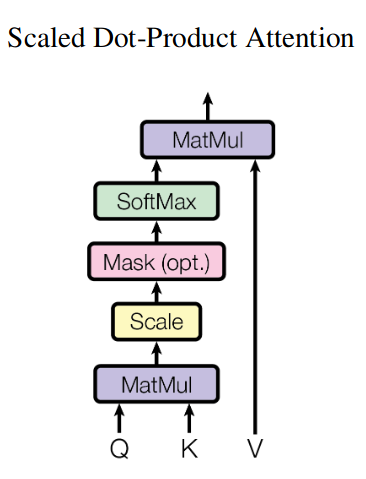
\includegraphics[scale=0.4]{images/att_dot_prod.png}}
\caption{\textRL{حساب تابع الانتباه عن طريق الجداء السلمي المقيس}
\textLR{\cite{Vaswani17}}}
\label{fig:att_dot_prod}
\end{figure}
إذ نلاحظ أن تابع الانتباه يتكون من مرحلتين، المرحلة الأولى هي حساب الـ
\textLR{score}
\begin{equation}
score(Q,K) = softmax(\frac{QK^T}{\sqrt{d_k}})
\end{equation}
والمرحلة الثانية هي تعديل مصفوفة القيم
$V$
بحسب قيم الـ
\textLR{score}.
إن دخل وخرج تابع الانتباه في المعادلة
\ref{eq:att}
هو عبارة عن مصفوفات.
\newline
ولفهم كيف يؤثر هذا التابع على كل شعاع
\textLR{token}
من أشعة الدخل،
نحسب الانتباه الذاتي للشعاع
$x_i$
من مصفوفة الدخل 
$X$.
بداية نحسب كل من قيمة
$k_i,q_i,v_i$
بحسب المعادلات
\ref{eq:att_mat_i}.
\begin{equation}
\begin{split}
&k_i = x_i W_k\\
&q_i = x_i W_q\\
&v_i = x_i W_v\\
\end{split}
\label{eq:att_mat_i}
\end{equation}
نحسب الجداء السلمي بين
$q_i$
وبين كل عنصر من عناصر المصفوفة
$K$ 
كما في المعادلات
\ref{eq:att_mat_i2}.
كما نعلم بأن الجداء السلمي يقيس مدى التشابه بين الشعاع
$q_i$
وبين أشعة المصفوفة
$K$.
ومن ثم نقيّس هذه القيم بتقسيمها على
$\sqrt{d_k}$،
حيث 
$d_k$
هو بعد النموذج 
%كما في الجدول 
%\ref{table:transformer_sympols}
أي بعد شعاع الدخل.
وقد وجد أن التقسيم على هذه القيمة جعل المشتق أكثر استقراراً
\textLR{\cite{illustratedTransformer}}.
ومن ثم بحساب الـ
\textLR{softmax}
والذي يضمن أن تكون القيم مقيسة بين
$[0,1]$،
خرج الـ
\textLR{softmax}
ندعوه بالـ
\textLR{score}.
 وقيم الـ
\textLR{score}
تحدد العناصر التي يجب التركيز عليها أثناء حساب خرج المرمز.
\begin{equation}
	\begin{split}
	&s_{11} = q_1.k_1\\
	&s_{12} = q_1.k_2\\
	&...\\
	&s_{1d} = q_1.k_d\\
	&score =score_1,score_2,..= softmax(\frac{s_{11}}{\sqrt{d_k}},\frac{s_{12}}{\sqrt{d_k}},...)\\
	\end{split}
	\label{eq:att_mat_i2}
\end{equation}
يوضح الشكل 
\ref{fig:att_score}
المرحلة الأولى من تابع الانتباه
\begin{figure}[H]
	\centerline{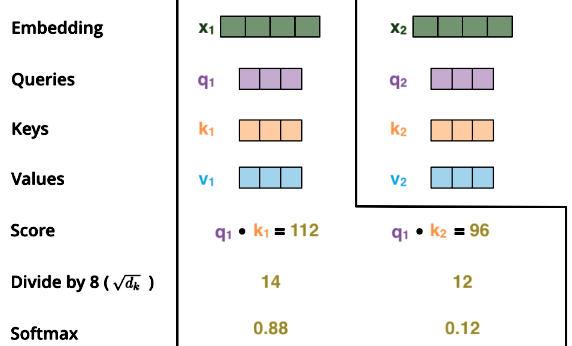
\includegraphics[scale=0.4]{images/att_score}}
	\caption{\textRL{ مثال رقمي عن حساب الـ}
		\textLR{score}
		\textRL{لتابع الانتباه عن طريق الجداء السلمي}
		\textLR{\cite{IllustratedAttention}}}
	\label{fig:att_score}
\end{figure}
المرحلة الثانية هي بحساب الخرج النهائي لتابع الانتباه
$z_1$
 وذلك بالتركيز على قيم 
$V$
بحسب التشابه بين 
$q,K$
كما في المعادلة 
\ref{eq:att_mat_fin}،
وكما يوضحه الشكل 
\ref{fig:att_output}،
وبالمثل نحسب
$z_2,z_3,...$.
\begin{equation}
z_1 = score_1.v_1 + score_2.v_2+....
\label{eq:att_mat_fin}
\end{equation}
\begin{figure}[H]
	\centerline{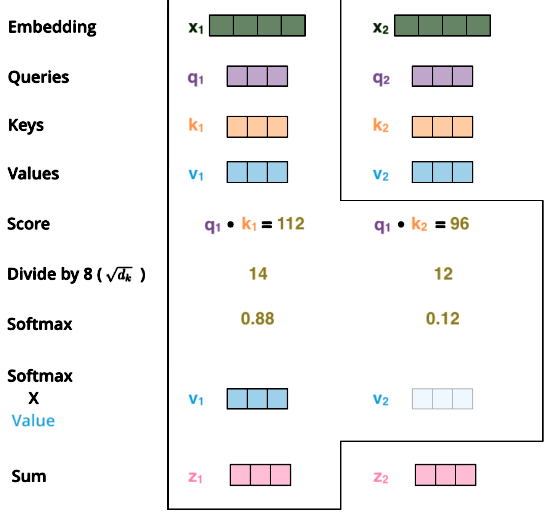
\includegraphics[scale=0.4]{images/attention_output.png}}
	\caption{\textRL{شكل توضيحي لحساب الانتباه من أجل كل عنصر دخل}
		\textLR{\cite{illustratedTransformer}}}
	\label{fig:att_output}
\end{figure}
%ونلاحظ من حساب الخرج أننا نقوم بالتركيز على قيم
%$V$
%بحسب التشابه بين 
%$q,K$.
%وبالمثل نحسب
%$z_2,z_3,...$.
%ويمكننا أن نحول الحساب إلى جداء مصفوفات مباشرة كما في معادلة حساب الانتباه 
%\ref{eq:att}.
\subsubsection{ الانتباه المتعدد الرؤوس
\textLR{Multi-head attention MHA}
}
إحدى الإضافات المهمة في نموذج المحول هي استخدام الانتباه المتعدد الرؤوس. وفيها يحسب الانتباه عدة مرات بحسب عدد الرؤوس
$h$
بشكل تفرعي، كما يوضحه الشكل
\ref{fig:MHA}
\begin{figure}[h!]
	\centerline{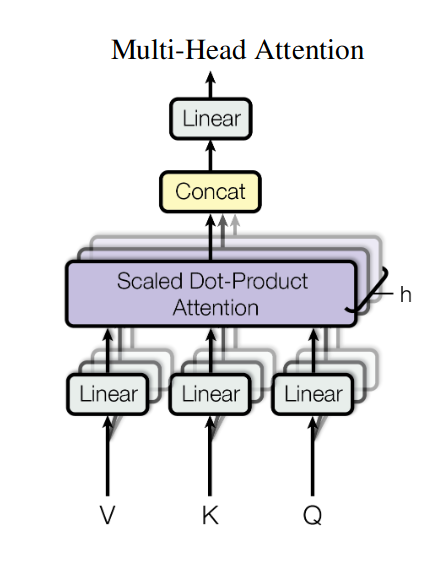
\includegraphics[scale=0.4]{images/MHA.png}}
	\caption{\textRL{الانتباه متعدد الرؤوس}
		\textLR{\cite{Vaswani17}}}
	\label{fig:MHA}
\end{figure}
يتم سَلسَلة (ضم)
\textLR{concatenate}
 خرج الرؤوس ضمن سلسلة واحدة، وعبر شبكة خطية من طبقة واحدة يتم تحويل أبعاد السلسلة إلى أبعاد النموذج من جديد عبر استخدام مصفوفة  الخرج
$W_0$.
\begin{equation}
\begin{split}
&MultiHead(Q,K,V) = Concat(head_1,...,head_H)W^O\\
&\text{\textLR{where  }} head_i = Attention(QW_i^Q,KW_i^K,VW_i^W)\\
\end{split}
\end{equation}
وبحسب
\textLR{\cite{Vaswani17}}،
فإن حساب الانتباه من أجل عدة رؤوس يسمح للنموذج بنمذجة معلومات السمات من مواقع مختلفة بشكل مشترك للرؤوس، وبعبارة أخرى معالجة سمات الدخل في عدة رؤوس يسمح لكل رأس أو نموذج انتباه بالتركيز على مجموعة معينة من السمات وهذا ما يفسر تحسن الأداء
\textLR{\cite{web:attention in cv}}.
في النموذج الأساسي
\textLR{\cite{Vaswani17}}
استخدمت توابع انتباه بعدد الرؤوس
$h = 8$
\subsubsection{الانتباه التقاطعي
\textLR{cross-attention}\label{MCHA}}
بالإضافة إلى حساب الانتباه الذاتي في مفكك الترميز
بين مداخله، فإنه أيضاً يُحسب
الانتباه بين المرمز ومفكك الترميز. نستخلص من خرج الطبقة الأخيرة من المرمز كل من الأشعة 
$V,K$،
ومن دخل طبقة مفكك الترميز نستخلص الشعاع 
$Q$.
\subsubsection{أنواع توابع الانتباه
\textLR{\cite{IllustratedAttention}}}
هناك عدة أنواع من التوابع لحساب
\textLR{score}
 الانتباه كما هو موضح في الشكل
\textLR{\ref{fig:att_types}}
 \begin{figure}[h!]
 	\centerline{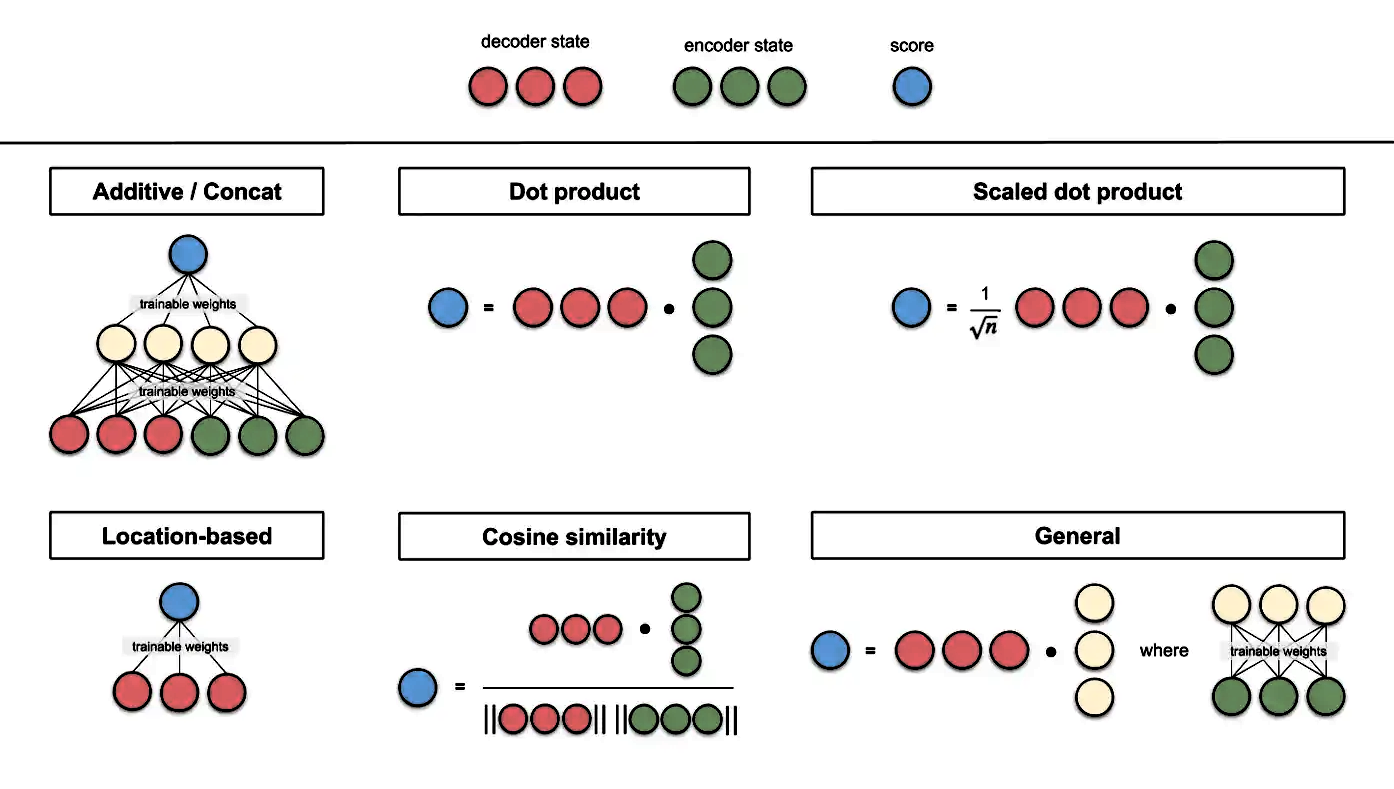
\includegraphics[width=\textwidth]{images/attention_types}}
 	\caption{\textRL{أنواع توابع الانتباه}
 	\textLR{\cite{IllustratedAttention}}}
 	\label{fig:att_types}
 \end{figure}

\begin{itemize}
	\item الانتباه الجمعي 
	$score(A,B) = v_\alpha^T tanh(W_a[A;B])$
	\item
	انتباه الجداء السلمي 
	$score(A,B) = A^TB$
	\item
	انتباه الجداء السلمي المقيس
	$score(A,B) = \frac{A^TB}{\sqrt{ns}}$
	وهو النوع المستخدم في نموذج المحول 
	\textLR{\cite{Vaswani17}}،
	حيث
	$n$
	هي بعد الشعاع
	$B$.
	\item الانتباه المعتمد على المحتوى
	$score(A,B) = cosine[A,B] = \frac{A.B^T}{||A||.||B||}$ 
	
	\item
	الانتباه العام
	$score(A,B) = A^TW_aB$


	
\end{itemize}